%%%%%%%%%%%%%%%%%%%%%%%%%%%%%%%%%%%%%%%%%%%%%%%%%%%%%%
% Thanks to Xu Minghao's work                        %
% I modify it into uchicago version                  %
% to not make new bug, I don't alter "Ritsumeikan"   %
% keywords in file. Pls feel free to use             %
%%%%%%%%%%%%%%%%%%%%%%%%%%%%%%%%%%%%%%%%%%%%%%%%%%%%%%

%%%%%%%%%%%%%%%%%%%%%%%%%%%%%%%%%%%%%%%%%%%%%%%%%%%%%%
% A Beamer template for Ritsumeikan University       %
% Author: Ming-Hao Xu (Xu Minghao)                   %
% Date:   April 2022.                                %
% LPPL Licensed.                                     %
%%%%%%%%%%%%%%%%%%%%%%%%%%%%%%%%%%%%%%%%%%%%%%%%%%%%%%

\documentclass[compress]{beamer}
\usepackage[utf8]{inputenc}
\usepackage[spanish]{babel}
\usepackage{amsmath}
\usepackage{amsfonts}
\usepackage{amssymb}
\usepackage{graphicx}
\usepackage{lipsum}
\usepackage{ragged2e}
\usepackage{hyperref}
\usepackage{float}
\usepackage{url}
\usepackage{multicol}
\usepackage{subfigure}
\usepackage{booktabs}
\usepackage{array}
\usepackage{multirow}

\usetheme{Berlin}
\useoutertheme{miniframes}
\setbeamertemplate{navigation symbols}{} 


\newcolumntype{N}{>{$}c<{$}}
\newcolumntype{D}{>{$}r<{$}}

\newcommand{\celda}[1]{
	\begin{minipage}{2.5cm}
		\vspace{5mm}
		#1
		\vspace{5mm}
	\end{minipage}
}

\author[Cristhian Moya Mota]{Cristhian Moya Mota}
\title[PE en Series Temporales]{Estudio sobre la Efectividad del Positional Encoding en Transformers para Series Temporales y Diseño de Mecanismos Adaptados}
\date{8 de septiembre de 2025} 

\logo{
\includegraphics[scale=0.04]{pic/logo}}
\institute[UGR]{
	\inst{}
	Tutor: Julián Luengo Martín\\Departamento de Ciencias de la Computación e Inteligencia Artificial\\
	\inst{ }
	Cotutor: Diego Jesús García Gil\\Departamento de Lenguajes y Sistemas Informáticos\\
	\vspace{2mm}	
}

\AtBeginSection[]
{
	\begin{frame}<beamer>{Contenido}
		\tableofcontents[currentsection,currentsubsection]
	\end{frame}
}


\begin{document}
	
	\begin{frame}
		\maketitle
	\end{frame}
	
	\begin{frame}{Contenido}
		\tableofcontents
	\end{frame}
	
	\setbeamerfont{footnote}{size=\tiny}
	\section{Introducción}
	
	\begin{frame}{Introducción}
		\begin{figure}
			\centering
			\begin{minipage}{0.4\textwidth}
				\centering
				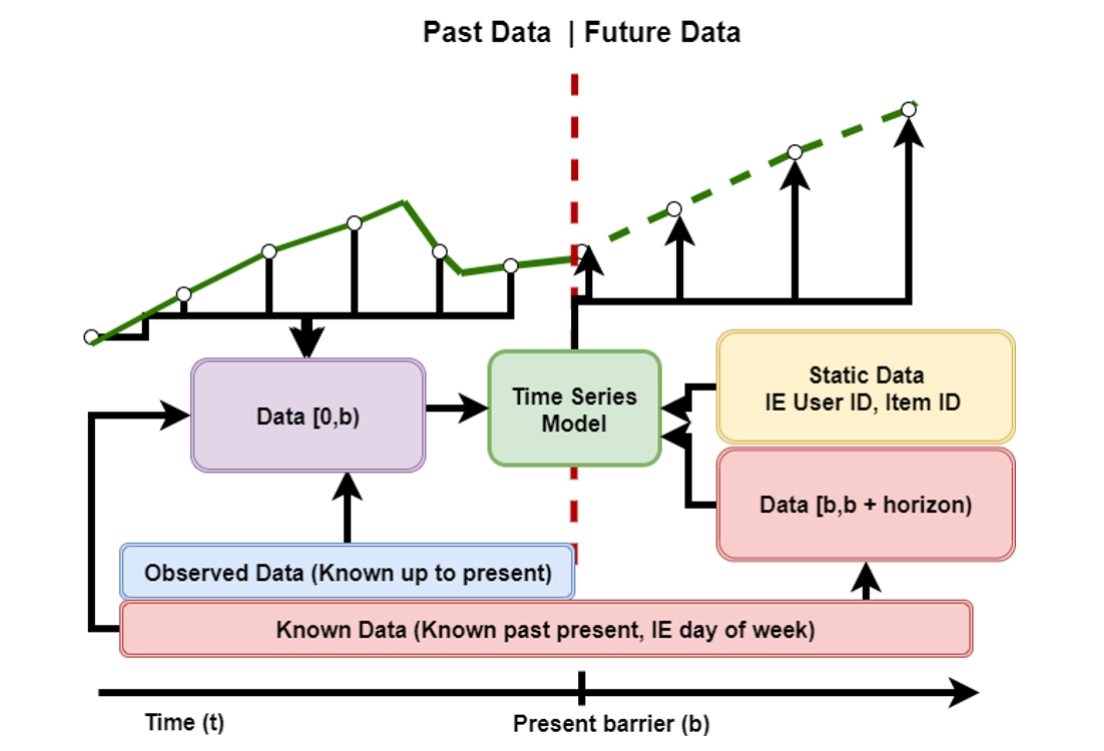
\includegraphics[height=\columnwidth]{pic/ts.png}
			\end{minipage}
			\hfill
			\begin{minipage}{0.4\textwidth}
				\centering
				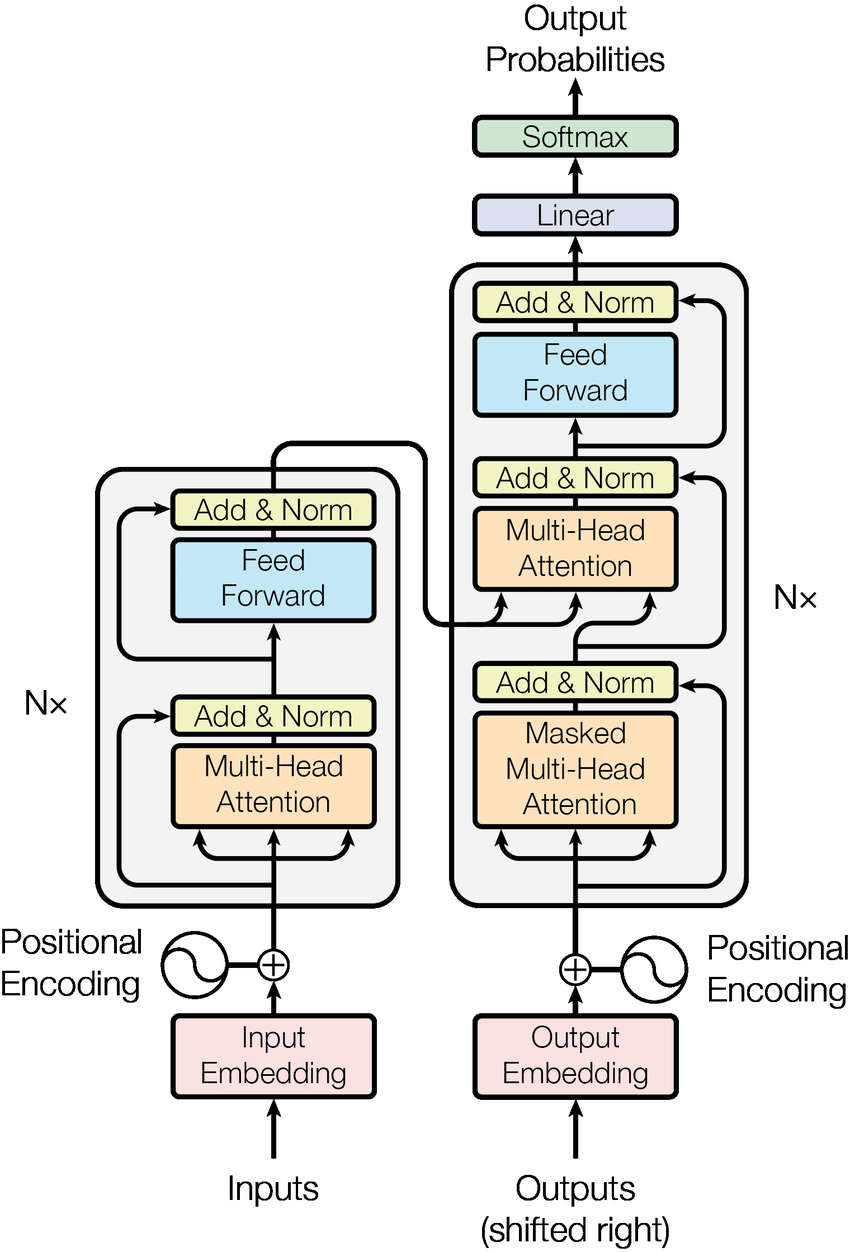
\includegraphics[height=\columnwidth]{pic/trans.png}
			\end{minipage}
			\caption[]{Forecasting en Series Temporales\footnote{{https://developer.nvidia.com/blog/time-series-forecasting-with-the-nvidia-time-series-prediction-platform-and-triton-inference-server/}}. Transformers\footnote{
					\url{https://doi.org/10.48550/arXiv.1706.03762}}}
		\end{figure}
	\end{frame}
	
	\begin{frame}{Introducción. Justificación}
		
		Aspectos que justifican la realización del proyecto:
		\begin{itemize}
			\item Falta de captura de la estructura. Ausencia de información semántica.
			\item Dificultad para adaptarse a diferentes escalas temporales y falta de semántica.
			\item Complejidad computacional y falta de interpretabilidad en la metodología.
		\end{itemize}
	\end{frame}
	
	\begin{frame}{Introducción. Objetivos}
		Este proyecto persigue:
		\begin{itemize}
			\item Comprender y exhibir las carencias de los métodos actuales.
			\item Proponer nuevos encodings para series temporales empleando Transformers.
			\item Evaluar la efectividad de las nuevas propuestas en diferentes ámbitos y conjuntos de datos.
			\item Identificar y establecer la base para nuevos métodos de codificación.
		\end{itemize}
	\end{frame}
	
	\section{Estado del arte}
	
	\begin{frame}{Estado del arte. Arquitecturas y PE}
		\begin{itemize}
			\item Métodos estadísticos: STL, ARIMA, Prophet.
			 
			\item Métodos basados en Transformer:
		
			\begin{itemize}
				\item Informer
				\item Autoformer
				\item FEDformer
			\end{itemize}
		\end{itemize}
		
		Problemas:
		\begin{enumerate}
			\item Escasa adición de información local.
			\item Mecanismos de atención poco cercanos a la semántica del dato.
		\end{enumerate}
		¿Solución? $\rightarrow$ Crear una nueva familia de codificaciones posicionales, capaz de captar información local y global.
	\end{frame}	 	
	\begin{frame}{Estado del arte. Caso particular de Informer}
		\begin{figure}
			\centering
			\begin{minipage}{0.55\textwidth}
				\centering
				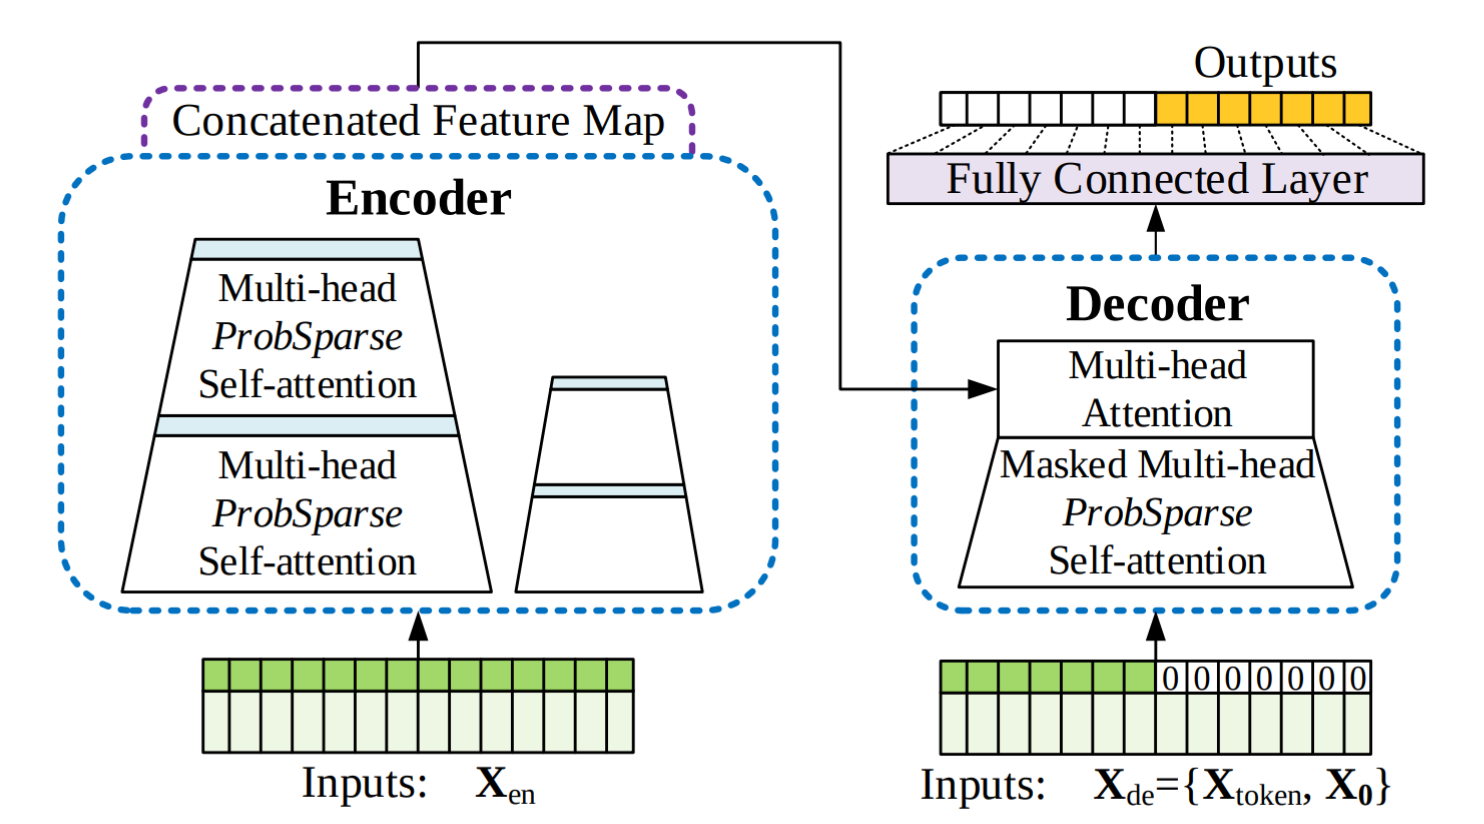
\includegraphics[width=\linewidth]{pic/informer.png}
			\end{minipage}
			\hfill
			\begin{minipage}{0.42\textwidth}
				\centering
				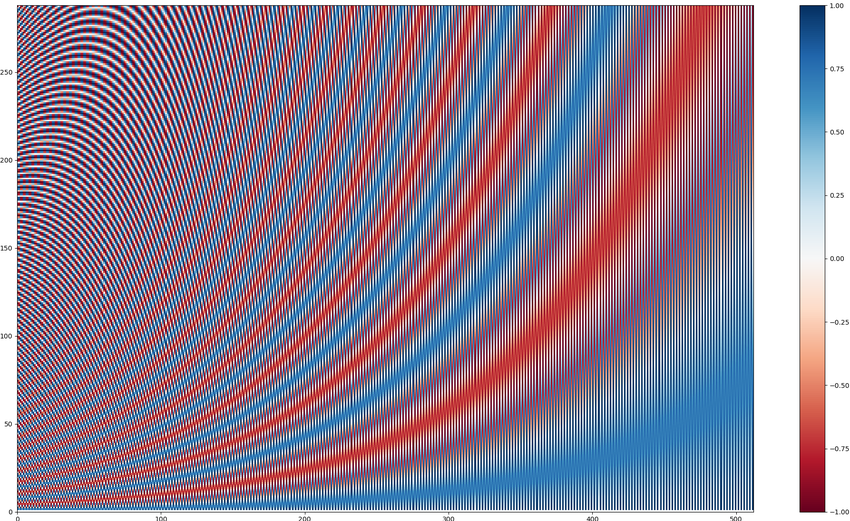
\includegraphics[width=\linewidth]{pic/encd}
			\end{minipage}
			\caption{Informer: arquitectura y encoding empleado\footnote{
					\url{https://doi.org/10.48550/arXiv.2012.07436}}}
		\end{figure}
	
	\end{frame}	 
		
	\section{Propuestas de PE}
	\begin{frame}{Encodings propuestos: Aspectos clave}
		Para mejorar la calidad del encoding, hay dos alternativas:
		\begin{itemize}
			\item Modificar el mecanismo de atención $\rightarrow$ pérdida de información local y complejidad añadida
			\item Modificar únicamente el PE $\rightarrow$ permite aprovechar arquitecturas existentes y trabajar directamente sobre el dato
		\end{itemize}
		
		Resultado: familia de modelos WinStat:
		\begin{enumerate}
			\item Sólo modificar la codificación posicional
			\item \emph{Concatenar} información en lugar únicamente sumarla
			\item \emph{Combinar PE existentes de manera ponderada} (normalizada con Softmax):
			
			 \end{enumerate}
	\end{frame}
	
	
	\begin{frame}
		\begin{figure}
			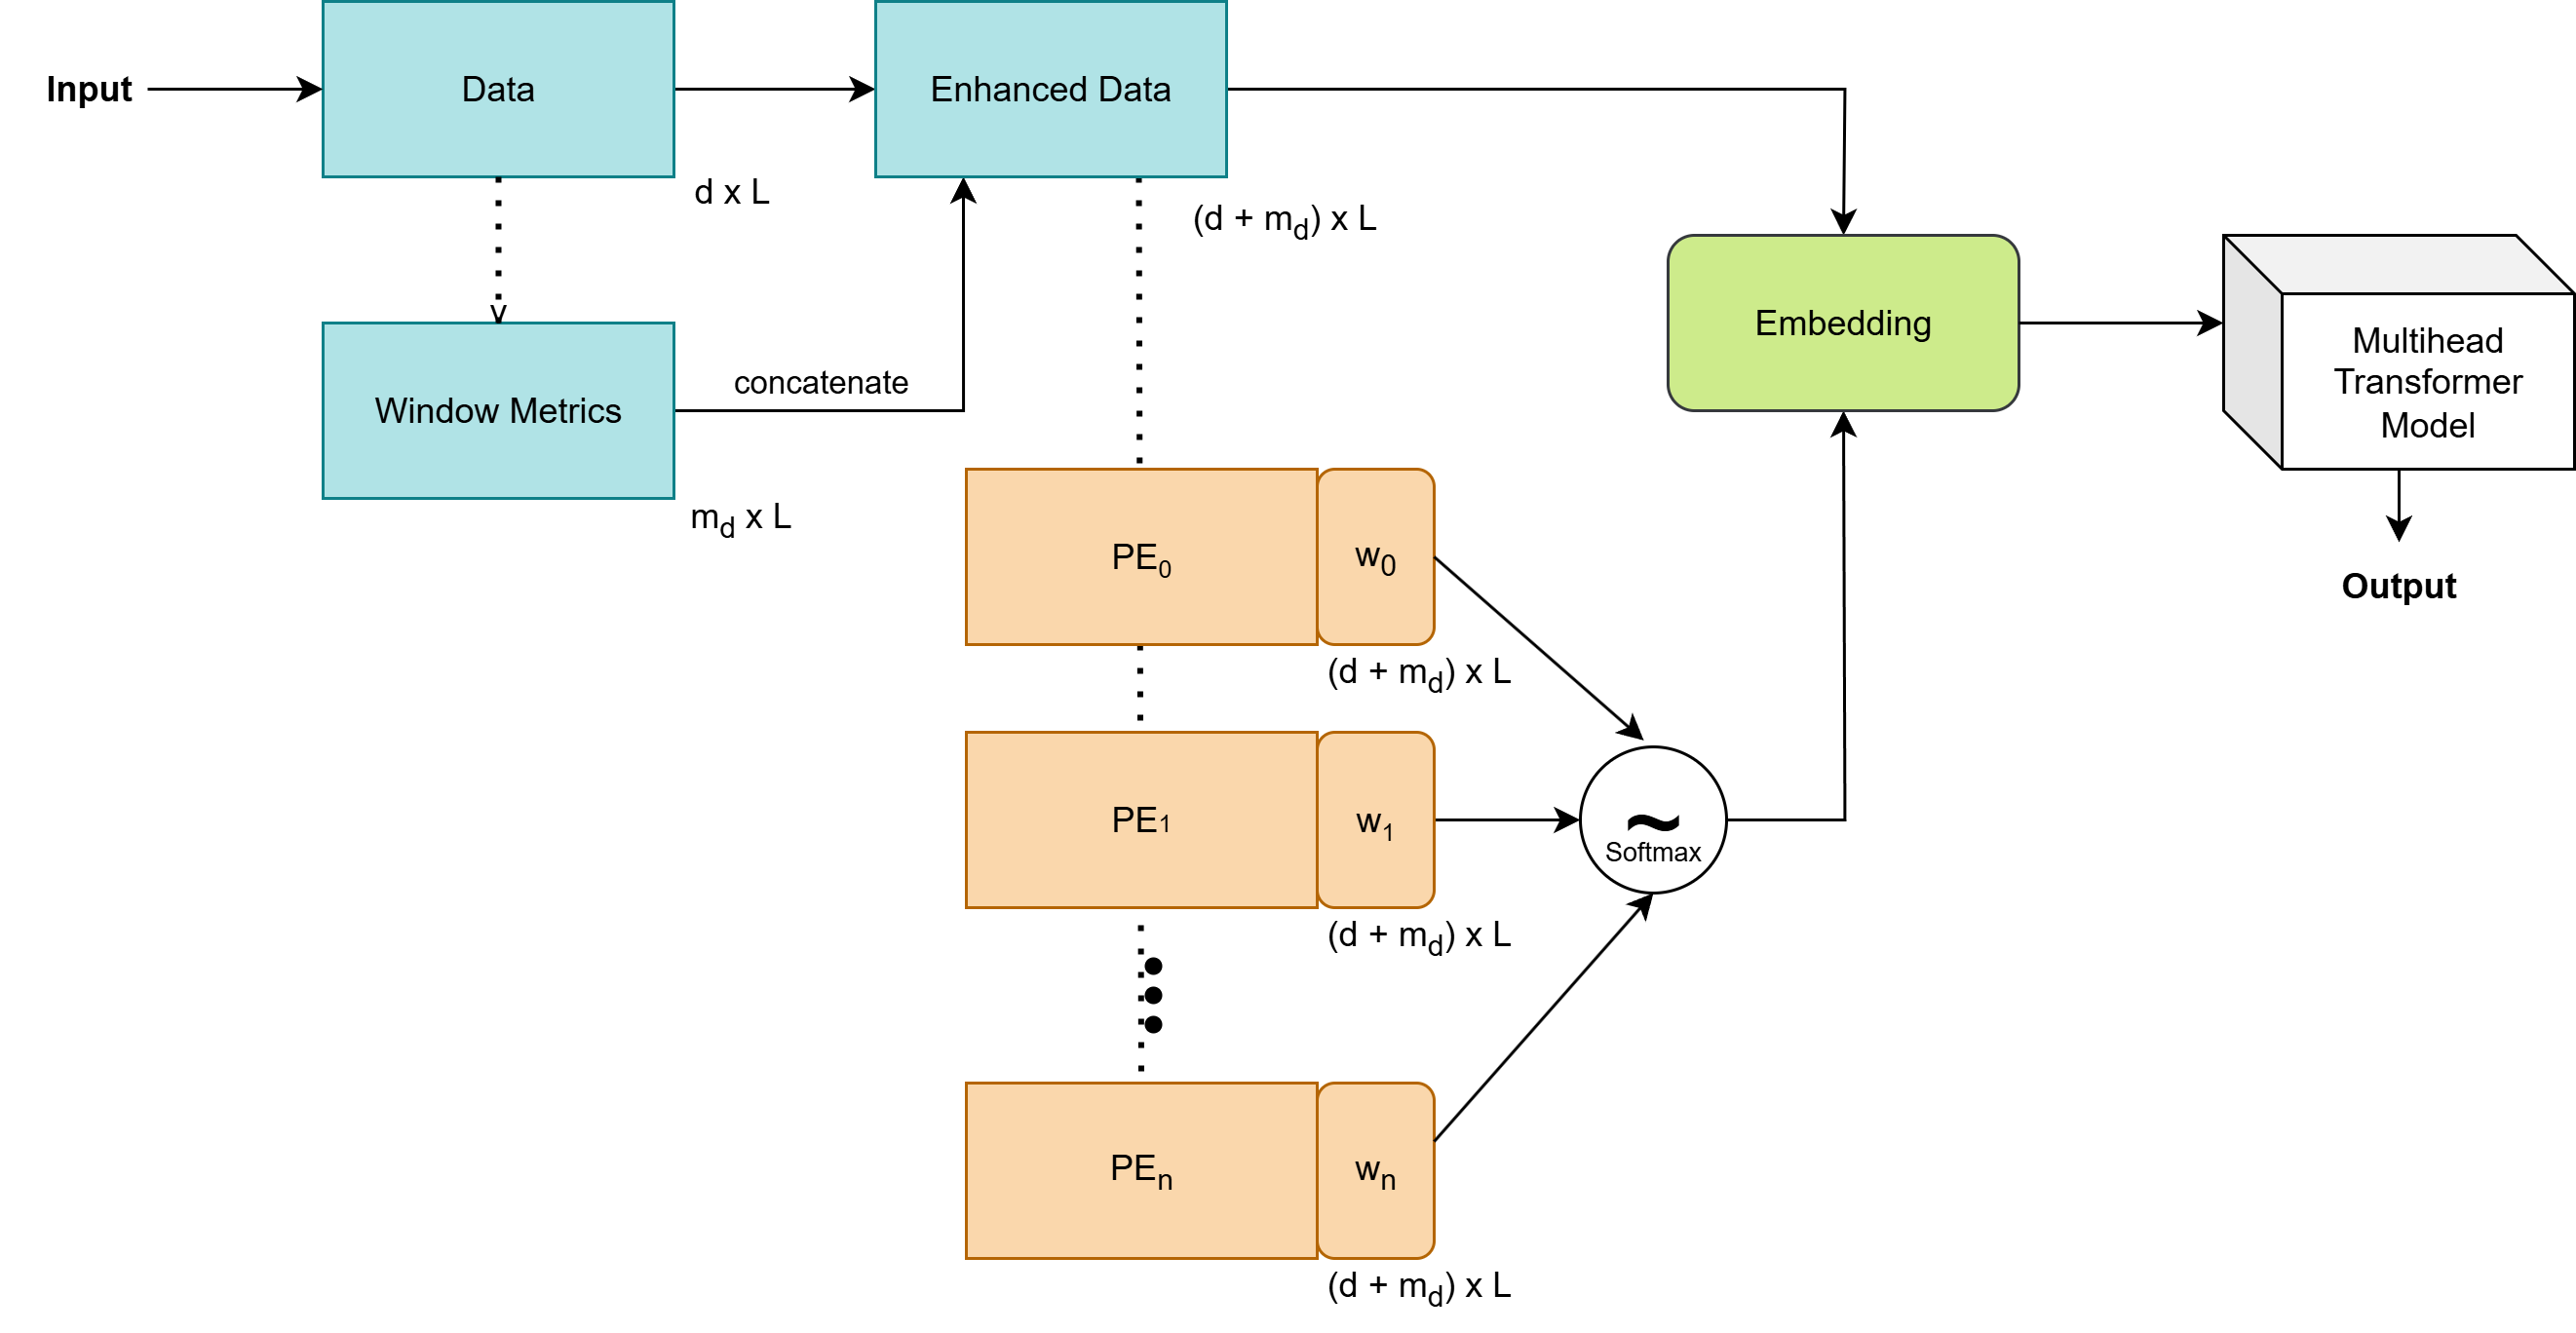
\includegraphics[width=\linewidth]{pic/enhancedhybrid.png}
		\end{figure}
		
	\end{frame}
	
	\begin{frame}{Encodings propuestos: \textbf{WinStat} (Variante base)}
	Ventana local de tamaño $W$ fijo, en cada posición $t$:
	
	\begin{itemize}
		\item \textit{Media}: $\mu_t = \frac{1}{|\mathcal{W}_t|} \sum_{x \in \mathcal{W}_t} x$
		\item \textit{Desviación estándar}: $\sigma_t = \sqrt{ \frac{1}{|\mathcal{W}_t|} \sum_{x \in \mathcal{W}_t} (x - \mu_t)^2 }$
		\item \textit{Mínimo}: $m^{\min}_t = \min_{x \in \mathcal{W}_t} x$
		\item \textit{Máximo}: $m^{\max}_t = \max_{x \in \mathcal{W}_t} x$
	\end{itemize}
	
	\[
	s_t = [\,\mu_t,\, \sigma_t,\, m^{\min}_t,\, m^{\max}_t\,] \in \mathbb{R}^{4}
	\]
	
	El embedding enriquecido de la posición $t$ es:
	
	\[
	\tilde{x}_t = [\,x_t \, \| \, s_t\,] \in \mathbb{R}^{d+4}
	\]
	
	\end{frame}
	
	\begin{frame}{Encodings propuestos: WinStatLag}
		
	Parte de WinStat, añadiendo $|\mathcal{L}|$ retardos especificados:
	
	\[
	s_t = [\,\mu_t,\, \sigma_t,\, m^{\min}_t,\, m^{\max}_t\,] \in \mathbb{R}^4
	\]
	
	Definimos para cada $\ell_j \in \mathcal{L}$:
	\[
	\delta_t^{(\ell_j)} = | x_t - x_{t - \ell_j}|, \quad \text{si } t - \ell_j \geq 1
	\]
	
	El \textit{embedding} enriquecido es la concatenación de $s_t$ y $\delta_t^{(\ell_j)}$
	\[
	\tilde{x}_t = [\,x_t \,\|\, s_t \,\|\, \delta_t^{(\ell_1)} \,\|\, \dots \,\|\, \delta_t^{(\ell_p)}\,] \in \mathbb{R}^{d + 4 + p}
	\]

	
	\end{frame}
	
	
	\begin{frame}{Encodings propuestos: WinStatFlex}
		
	Basado en WinStatLags, añadiendo la información ponderada de:
	\begin{enumerate}
	\item Encoding sinusoidal original
	\item LPE:
	
	$$
	LPE_{(pos)} = W_{pos}, \quad W_{pos} \in \mathbb{R}^d
	$$
	
	$$
	X_{LPE} = \tilde{x}_t + LPE[pos]
	$$
	
	\item TAPE:
	
	\begin{equation}
		\centering
		\omega^{new}_k = k \cdot \frac{d_{model}}{L}
	\end{equation}
	
	
	\begin{equation}
		\begin{aligned}
			\text{TAPE}_{(pos,2i)} &= \sin\!\left( pos \cdot \omega^{new}_i \right) \\
			\text{TAPE}_{(pos,2i+1)} &= \cos\!\left( pos \cdot \omega^{new}_i \right)
		\end{aligned}
	\end{equation}
	
	$$
	X_{TAPE} = \tilde{x}_t + TAPE[pos]
	$$
	
		\end{enumerate}
	\end{frame}
	
	\begin{frame}{Encodings propuestos: WinStatTPE}
	\begin{itemize}
		\item Emplea WinStatFlex como base
		\item Sustituye TAPE por TPE:
		
		$$S(i, j) = \exp\left( -\frac{\|x_i - x_j\|^2}{2\sigma^2} \right)$$
		
		Añadiéndose al encoding sinusoidal original la nueva componente:
		
		$$T\text{-}PE(i) = PE(i) + S(i, j)$$
		
		$$
		X_{TPE} = \tilde{x}_t + T-PE[pos]
		$$
		
		
	 \end{itemize}
	\end{frame}
	
	\section{Evaluación de PE mediante conjuntos de datos}
	
	\begin{frame}{Evaluación. Conjuntos de datos}
		Conjuntos de datos para la evaluación:
		
		\begin{columns}
			
			\column{0.4\linewidth}
			\begin{itemize}
				\item Household Power Consumption (HPC)
				\item ETTh1
				\item ETTh2
				\item Yellow Trip Data
				\item TINA
			\end{itemize}
		
			\column{0.6\linewidth}
			\centering
			\begin{figure}
				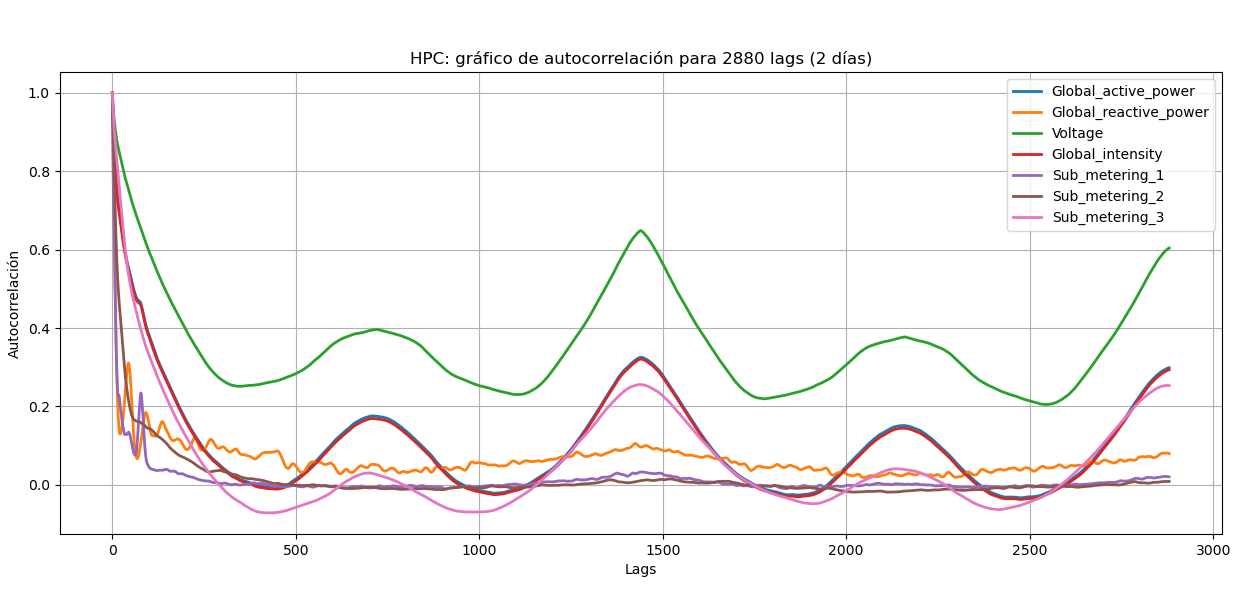
\includegraphics[width=\linewidth]{pic/auto.png}
				\caption{Autocorrelación de Household Power Consumption}
			\end{figure}
		
		\end{columns} 
				
	\end{frame}
	
	\begin{frame}{Evaluación. Condiciones de entrenamiento}
		\begin{columns}
			\column{0.55\linewidth}
			\begin{enumerate}
				\item Resultado a partir de ejecuciones múltiples promedio (semilla \textit{random})
				\item Ejecución de encoding barajado para comprobar alcance de su aportación en cada modelo.
				\item Métricas: MSE y MAE
				\item Heurística para el tamaño de ventana: entre 1/3 y 1/4 de longitud de secuencia.
			\end{enumerate}
			
			\column{0.45\linewidth}
			\centering
			\begin{figure}
				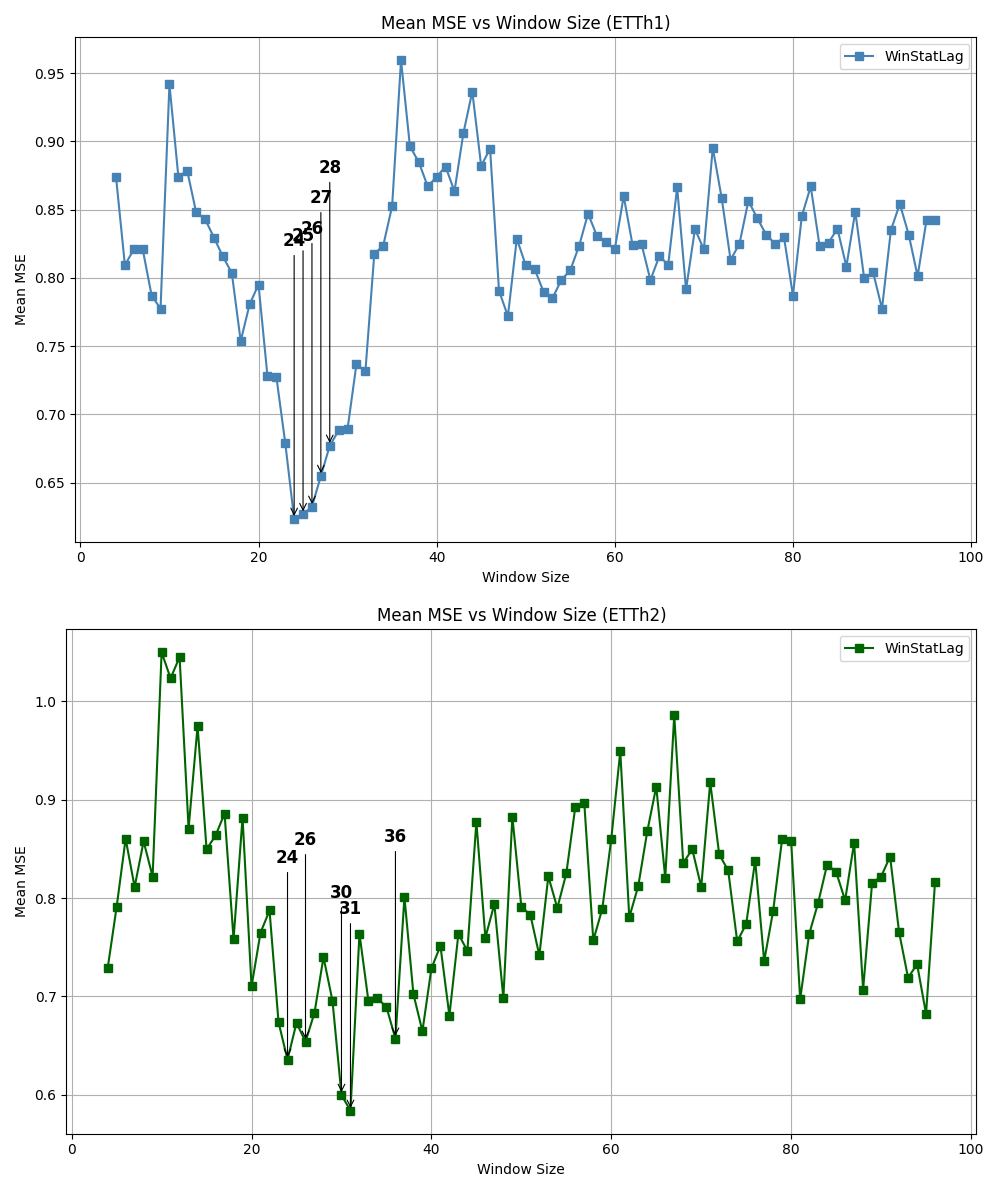
\includegraphics[height=\columnwidth]{pic/wind.png}
				\caption{Elección del tamaño de ventana}
			\end{figure}
			
		\end{columns} 
		
		
	\end{frame}
	
	\subsection{}
	\begin{frame}{Evaluación. Household Power Consumption (I)}	
		\begin{figure}
			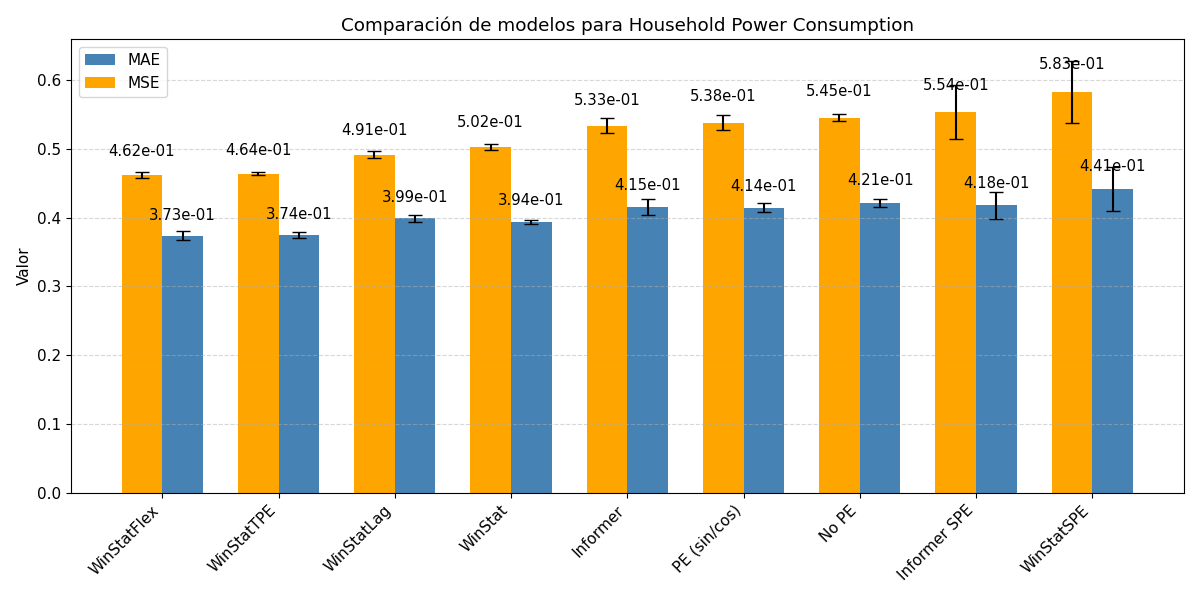
\includegraphics[width=\linewidth]{pic/hpcgraph.png}
			\caption{Resultados de Household Power Consumption}
		\end{figure}
	\end{frame}
	
		\begin{frame}{Evaluación. Household Power Consumption (II)}	
		\begin{figure}
			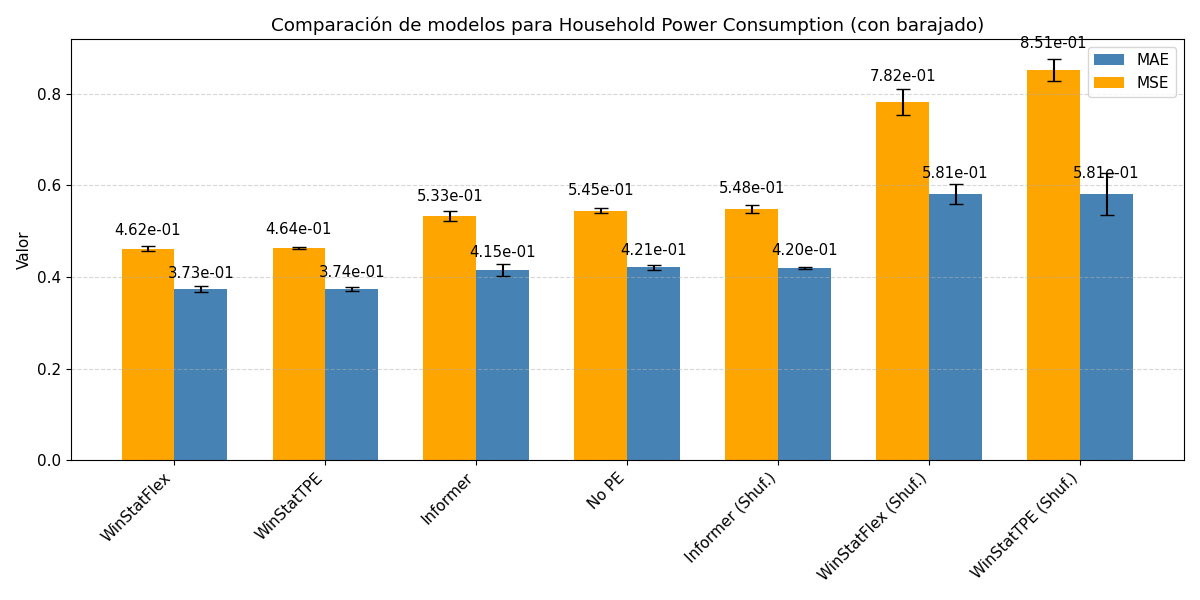
\includegraphics[width=\linewidth]{pic/hpcgraphshuffled.png}
			\caption{Resultados de HPC, con barajado en el PE}
		\end{figure}
	\end{frame}
	
	
	\begin{frame}{Evaluación. Household Power Consumption (III)}
		
		\begin{table}[ht]
		\centering
		\resizebox{\textwidth}{!}{%
		\begin{tabular}{l|N N|N N}

			\toprule
			Modelo & \text{MAE (Media)} & \text{MAE (STD)} & \text{MSE (Media)} & \text{MSE (STD)} \\
			\midrule
			WinStatFlex & 0,373488 & 0,006858 & 0,461892 & 0,004841 \\
			WinStatTPE & 0,374392 & 0,004132 & 0,463651 & 0,001917 \\
			Informer & 0,415272 & 0,012216 & 0,532965 & 0,010976 \\
			No PE & 0,421343 & 0,005856 & 0,544844 & 0,005447 \\
			Informer (Shuffled) & 0,419960 & 0,002769 & 0,548443 & 0,009148 \\
			WinStatFlex (Shuffled) & 0,581124 & 0,021991 & 0,782092 & 0,027368 \\
			WinStatTPE (Shuffled) & 0,581001 & 0,046717 & 0,851115 & 0,024083 \\
			\bottomrule
		\end{tabular}}
		\label{hpcresultados_modelos}
	\end{table}
	\end{frame}
	
	\subsection{ETTh1}
	\begin{frame}{Evaluación. ETTh1 y ETTh2 (I)}

	\begin{figure}
		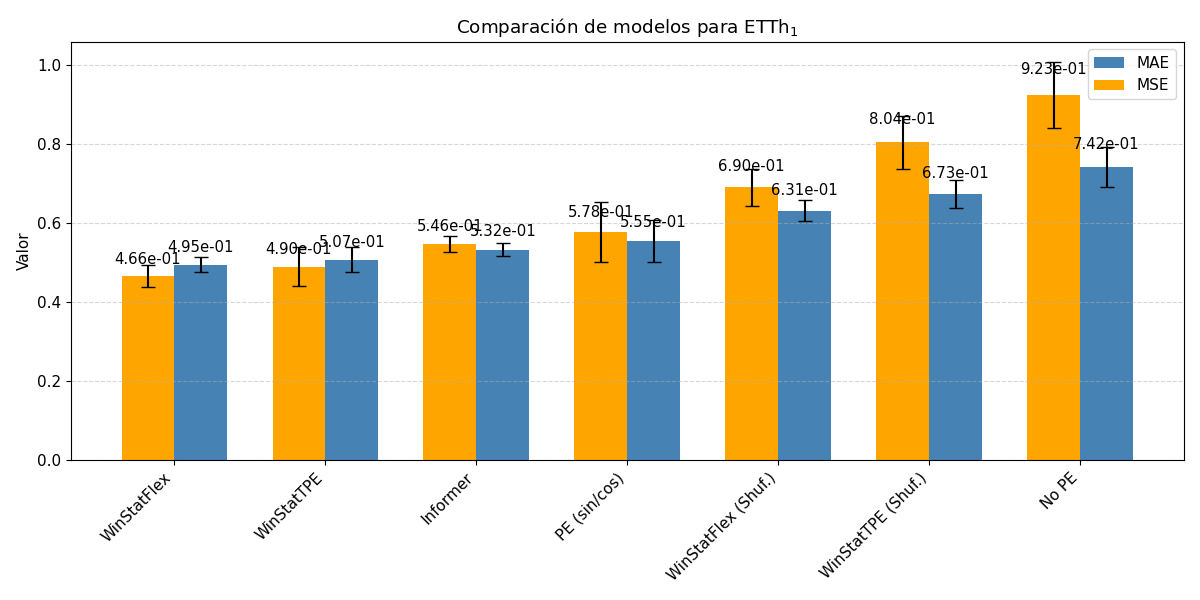
\includegraphics[scale=0.225]{pic/etth1fin.png}
	\end{figure}
	
	\begin{table}
	\centering

	\resizebox{!}{0.14\textheight}{%

	\begin{tabular}{l|NN|NN}
		\toprule
		Modelo & \text{MAE (Media)} & \text{MAE (STD)} & \text{MSE (Media)} & \text{MSE (STD)} \\
		\midrule
		WinStatFlex            & 0,4947 & 0,0195 & 0,4660 & 0,0277 \\
		WinStatTPE             & 0,5072 & 0,0312 & 0,4896 & 0,0482 \\
		Informer               & 0,5324 & 0,0171 & 0,5458 & 0,0204 \\
		PE (sin/cos)           & 0,5552 & 0,0531 & 0,5776 & 0,0755 \\
		WinStatFlex (Shuf.)    & 0,6313 & 0,0276 & 0,6897 & 0,0461 \\
		WinStatTPE (Shuf.)     & 0,6728 & 0,0358 & 0,8036 & 0,0667 \\
		No PE                  & 0,7419 & 0,0509 & 0,9235 & 0,0841 \\
		\bottomrule
	\end{tabular}}	
	\end{table}
	
	\end{frame}


	\subsection{ETTh2}
	\begin{frame}{Evaluación. ETTh1 y ETTh2 (II)}
		
		\begin{figure}
			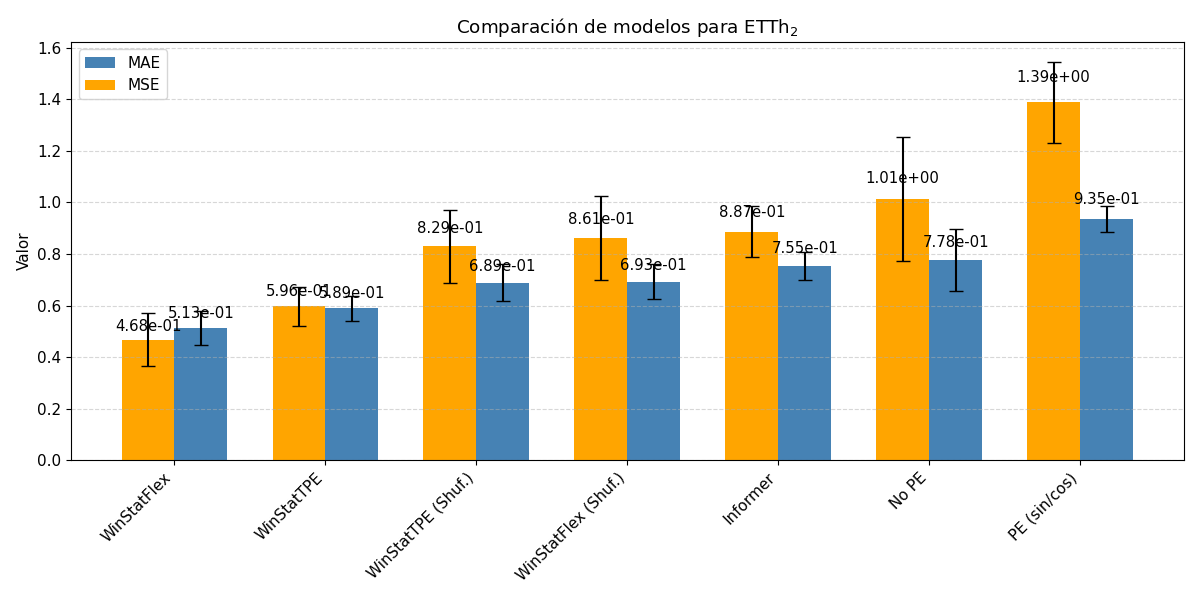
\includegraphics[scale=0.225]{pic/etth2fin.png}
		\end{figure}
		
		\begin{table}
			\centering
			
			\resizebox{!}{0.14\textheight}{%
				
			\begin{tabular}{l|NN|NN}
			\toprule
			Modelo & \text{MAE (Media)} & \text{MAE (STD)} & \text{MSE (Media)} & \text{MSE (STD)} \\
			\midrule
			WinStatFlex            & 0,5128 & 0,0651 & 0,4677 & 0,1018 \\
			WinStatTPE             & 0,5889 & 0,0496 & 0,5964 & 0,0760 \\
			WinStatTPE (Shuf.)     & 0,6892 & 0,0714 & 0,8294 & 0,1418 \\
			WinStatFlex (Shuf.)    & 0,6929 & 0,0671 & 0,8608 & 0,1625 \\
			Informer               & 0,7549 & 0,0540 & 0,8866 & 0,1001 \\
			No PE                  & 0,7777 & 0,1199 & 1,0132 & 0,2417 \\
			PE (sin/cos)           & 0,9355 & 0,0514 & 1,3881 & 0,1582 \\
			\bottomrule
		\end{tabular}
				
				}	
		\end{table}
		
	\end{frame}
	
	\subsection{}
	
	\begin{frame}{Evaluación. Yellow Trip Data (I)}
		
		\begin{table}[!ht]
			\centering
			\resizebox{\textwidth}{!}{%
				
			\begin{tabular}{l|cc|cc}
				\toprule
				Modelo & MSE (Media) & MSE (STD) & MAE (Media) & MAE (STD) \\
				\midrule
				WinStatTPE & $1,0 \times 10^{-5}$ & $5,0 \times 10^{-6}$ & $2,547 \times 10^{-3}$ & $9,37 \times 10^{-4}$ \\
				WinStatFlex & $1,7 \times 10^{-5}$ & $8,0 \times 10^{-6}$ & $3,529 \times 10^{-3}$ & $1,027 \times 10^{-3}$ \\
				Informer & $1,9 \times 10^{-5}$ & $7,0 \times 10^{-6}$ & $3,987 \times 10^{-3}$ & $7,95 \times 10^{-4}$ \\
				PE (sin/cos) & $2,4 \times 10^{-5}$ & $1,0 \times 10^{-5}$ & $4,307 \times 10^{-3}$ & $1,044 \times 10^{-3}$ \\
				No PE & $4,6 \times 10^{-5}$ & $6,0 \times 10^{-5}$ & $4,626 \times 10^{-3}$ & $3,954 \times 10^{-3}$ \\
				WinStatTPE (Shuf.) & $5,6 \times 10^{-5}$ & $6,3 \times 10^{-5}$ & $5,688 \times 10^{-3}$ & $3,983 \times 10^{-3}$ \\
				WinStatFlex (Shuf.) & $1,302 \times 10^{-1}$ & $1,838 \times 10^{-1}$ & $7,203 \times 10^{-2}$ & $9,583 \times 10^{-2}$ \\
				\bottomrule
			\end{tabular}}

			\label{taxifinal}
		\end{table}
		
	\end{frame}
	
	\begin{frame}{Evaluación. Yellow Trip Data (II)}
			\begin{figure}
			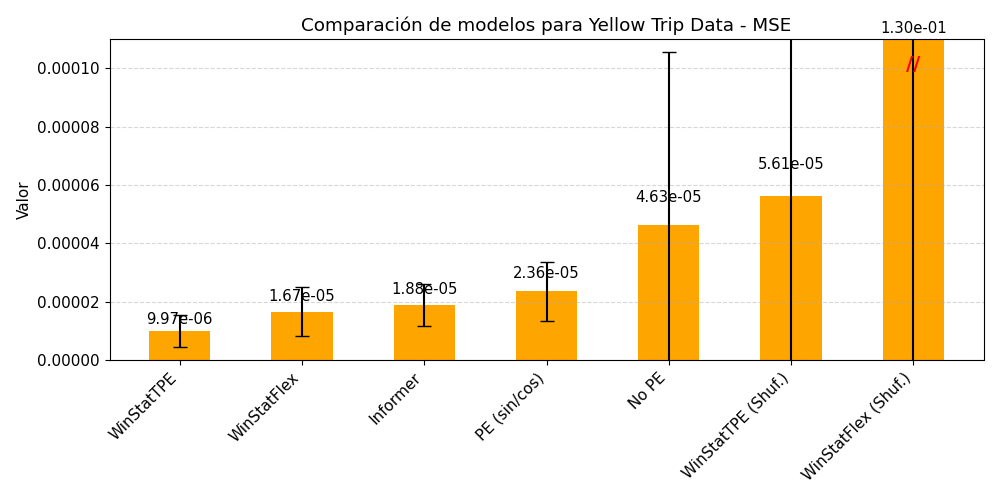
\includegraphics[scale=0.26]{pic/taxifinalmse.png}
		\end{figure}
		
		\begin{figure}
			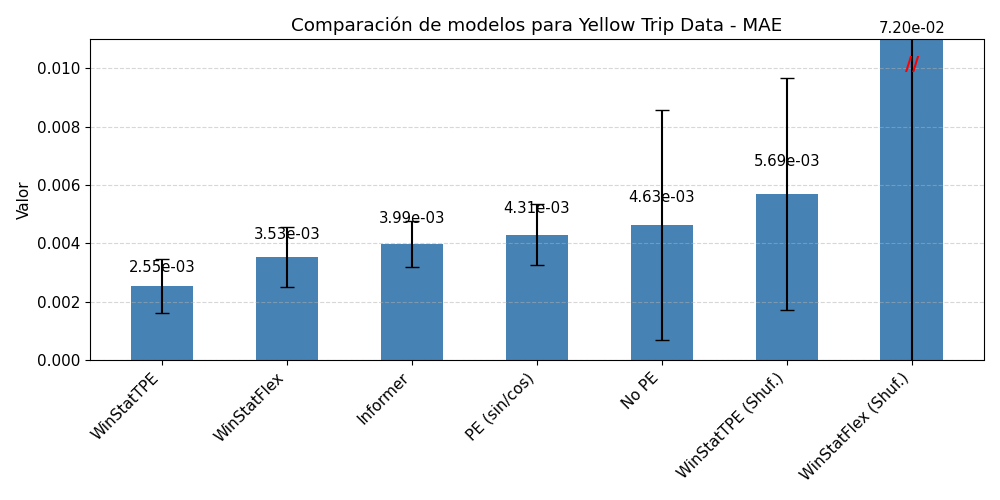
\includegraphics[scale=0.26]{pic/taxifinalmae.png}
		\end{figure}
	\end{frame}


	\begin{frame}{Evaluación. TINA}
		
		
		\begin{figure}
			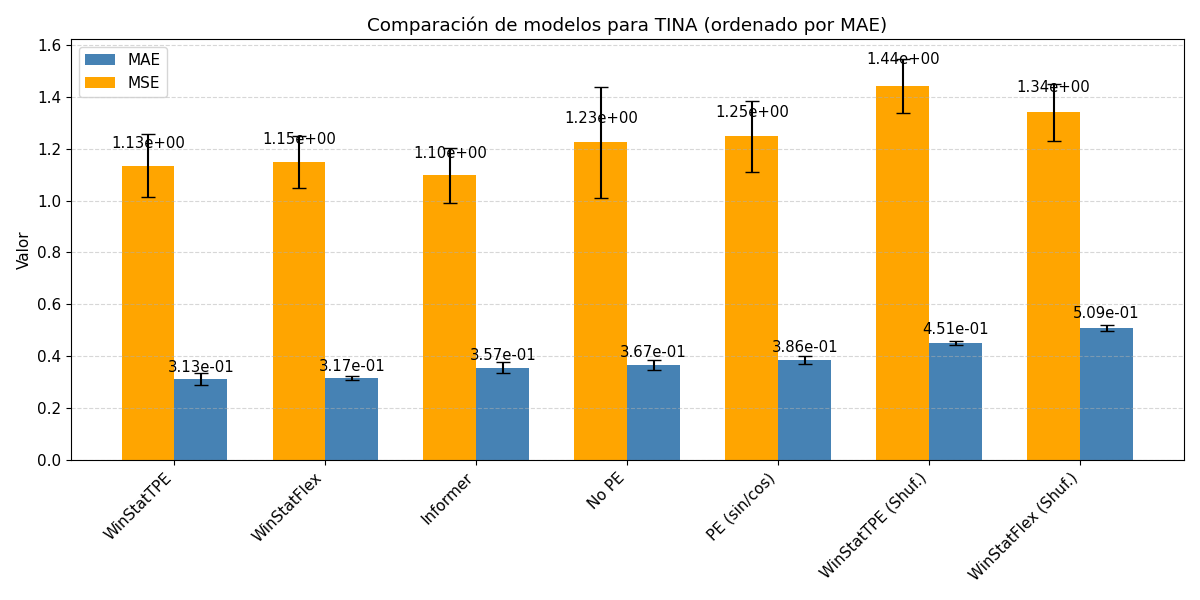
\includegraphics[scale=0.25]{pic/tinafinal2.png}
		\end{figure}
		
		\begin{table}
			\centering
			
			\resizebox{!}{0.14\textheight}{%
				\begin{tabular}{l|NN|NN}
					\toprule
					Modelo & \text{MSE (Media)} & \text{MSE (STD)} & \text{MAE (Media)} & \text{MAE (STD)} \\
					\midrule
					Informer & 1,0965 & 0,1064 & 0,3566 & 0,0200 \\
					WinStatTPE & 1,1334 & 0,1216 & 0,3126 & 0,0215 \\
					WinStatFlex & 1,1481 & 0,1012 & 0,3170 & 0,0070 \\
					No PE & 1,2251 & 0,2137 & 0,3665 & 0,0179 \\
					PE (sin/cos) & 1,2470 & 0,1375 & 0,3861 & 0,0164 \\
					WinStatFlex (Shuf.) & 1,3399 & 0,1100 & 0,5094	 & 0,1025 \\
					WinStatTPE (Shuf.) & 1,4412 & 0,1025 & 0,4511 & 0,0061 \\
					\bottomrule 
				\end{tabular}
				
			}	
		\end{table}
		
	\end{frame}
	
\begin{frame}{Evaluación. Resultados finales}
	\begin{table}
		\centering
		\resizebox{\linewidth}{!}{%
			\setlength{\tabcolsep}{7pt}%
			\renewcommand{\arraystretch}{1.3}%
			\begin{tabular}{c|cccccccccc}
				\toprule
				\multirow{2}{*}{\parbox{2cm}{\centering Modelo \\ Métrica}} 
				& \multicolumn{2}{c}{Informer} 
				& \multicolumn{2}{c}{PE (sin/cos)} 
				& \multicolumn{2}{c}{WinStatFlex} 
				& \multicolumn{2}{c}{WinStatTPE} 
				& \multicolumn{2}{c}{No PE} \\
				\cmidrule(lr){2-3}\cmidrule(lr){4-5}\cmidrule(lr){6-7}\cmidrule(lr){8-9}\cmidrule(lr){10-11}
				& MSE & MAE & MSE & MAE & MSE & MAE & MSE & MAE & MSE & MAE \\
				\midrule
				HPC   & $0.5329$ & $0.4152$ & $0.5377$ & $0.4140$ & $\mathbf{0.4618}$ & $\mathbf{0.3734}$ & $0.4636$ & $0.3743$ & $0.5448$ & $0.4213$ \\
				ETTh1 & $0.5458$ & $0.5324$ & $0.5776$ & $0.5552$ & $\mathbf{0.4660}$ & $\mathbf{0.4947}$ & $0.4896$ & $0.5072$ & $0.9235$ & $0.7419$ \\
				ETTh2 & $0.8866$ & $0.7549$ & $1.3881$ & $0.9355$ & $\mathbf{0.4677}$ & $\mathbf{0.5128}$ & $0.5964$ & $0.5889$ & $1.0132$ & $0.7777$ \\
				Yellow Trip & $1.9\times10^{-5}$ & $3.987\times10^{-3}$ & $2.4\times10^{-5}$ & $4.307\times10^{-3}$ & $1.7\times10^{-5}$ & $3.529\times10^{-3}$ & $\mathbf{1.0\times10^{-5}}$ & $\mathbf{2.547\times10^{-3}}$ & $4.6\times10^{-5}$ & $4.626\times10^{-3}$ \\
				TINA  & $\mathbf{1.0965}$ & $0.3566$ & $1.2470$ & $0.3861$ & $1.1481$ & $0.3170$ & $1.1334$ & $\mathbf{0.3126}$ & $1.2251$ & $0.3665$ \\
				\midrule\midrule
				Count & \multicolumn{2}{c}{1} & \multicolumn{2}{c}{0} & \multicolumn{2}{c}{\textbf{6}} & \multicolumn{2}{c}{3} & \multicolumn{2}{c}{0} \\
				\bottomrule
			\end{tabular}}
		\caption{Resumen de resultados finales}
		\label{resumenfinal}
	\end{table}
\end{frame}
		
	
\section{Conclusiones}
\subsection{Conclusiones}
\begin{frame}{}
		El proyecto ha conseguido:
		\begin{itemize}
			\item Detectar el principal problema de la falta de localidad, asociada al encoding escaso proporcionado por el enfoque tradicional.
			\item Ofrecer un conjunto de modelos que demuestran una mejora considerable de los resultados.
			\item Demostrar empíricamente los resultados en varios conjuntos de datos sobre los que han sido evaluados.
			\item Proponer un enfoque sencillo de comprender,  mediante estadísticos básicos y ponderaciones normalizadas.
			\item Obtener, del conjunto de propuestas, un modelo novedoso y versátil, WinStatFlex, gracias a la creación de un entorno de pruebas estable.
		\end{itemize}
	
\end{frame}


\subsection{Trabajos futuros}
\begin{frame}{}

\begin{itemize}
	\item Aplicación de las técnicas expuestas en la clasificación de series temporales.
	\item Adaptación de los mecanismos de localidad para su uso en la detección de anomalías\footnote{https://timeeval.github.io/evaluation-paper/}
	\item Mejorar el aprovechamiento de recursos: aprendizaje federado para la optimización de recursos y privacidad del dato.
\end{itemize}


\begin{figure}
	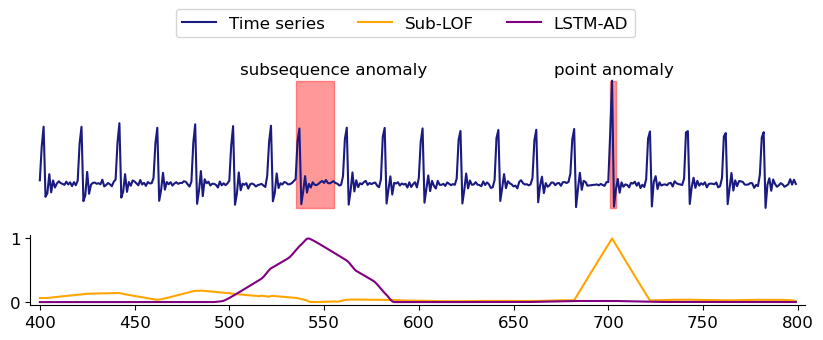
\includegraphics[scale=0.3]{pic/anomaly.png}
\end{figure}
	
\end{frame}


\begin{frame}
	\centering \textbf{Gracias}

	\begin{figure}[H,font=\Small]
		\centering
		\subfigure{
\includegraphics[width=0.25\textwidth]{pic/QRTFM}} 
		\label{fig:calidad}
		
		¿Preguntas?
		
	\end{figure}
	
	
\end{frame}


\end{document}